\documentclass[]{article}

\usepackage[margin=1in]{geometry}

\usepackage[]{amsthm}
\usepackage[parfill]{parskip}
\usepackage[]{graphicx}
\graphicspath{{../img/}}

\title{CMSC 510: Disjoint Set Data Structures}
\author{Acacia Ackles}

\begin{document}
    
\maketitle

Lecture notes adapted from \textit{Introduction to Algorithms 4e}, Cormen, Leiserson, Rivest, and Stein.

\section*{From Algorithms to Data Structures}

    So far we have been talking about ways to analyze general kinds of algorithms, both iterative and recursive. These general analysis techniques can be very powerful tools to have in your toolkit for analyzing algorithms and finding places where they could be more efficient. 
    
    However, you probably recall from 270 that all the algorithmic techniques in the world won't save you if you have a bad data structure. For example, you can never do any better than $O(n)$ search in an unsorted list; it's just not possible. So choosing, or in some cases constructing, a good data structure can be just as essential as understanding algorithmic properties.
    
    Today instead we'll be diving into data structures, in particular a case study on a data structure that will allow us to quickly perform some key operations. 

\section*{Motivation}

    You're a student at Lawrence University (hello!). You're a computer science student, so you're interested in doing things efficiently and logically, even if they require a lot of extra work up front. 

    One thing you'd like to do as efficiently as possible is get to your various classes. Here, we mean efficiently in the sense of heat efficiency: in Wisconsin, the winters can be terribly cold. So you'd like to know which buildings are connected to one another, so that you can avoid stepping outside as much as possible while you're moving from class to class.
    
    College campuses also have a lot of construction happening on them at all times, so it's possible that both the list of buildings and the list of connections could change at any time. You want to make sure that you can easily update your knowledge of which buildings are connected to each other. 

\subsection*{Problem}

    Given a list of buildings:

    \begin{verbatim}
        Briggs
        Steitz
        Youngchlid
        Warch
        Commmons
        Main
        Wriston
    \end{verbatim}

    And a list of connections between buildings:

    \begin{verbatim}
        Briggs <-> Steitz
        Steitz <-> Youngchild
        Warch <-> Commmons
        Briggs <-> Youngchild
        Steitz <-> Wriston
    \end{verbatim}

    Can you come up with a data structure in which to store these buildings that will make the following operations \textbf{as fast as possible}? 

    \begin{enumerate}
        \item Given the names of two buildings, find out if they are connected.
        \item Given a new building and new connections, update your data structure.
    \end{enumerate}

    \textit{NB: Your data structure does not have to store information on whether the connections are direct or through another building. It can treat both of those cases in the same way.}

    \subsection*{Solution?}

    What you might quickly find is that those simple structures you are used to which might be good at doing one of these things are not terribly good at doing both of those things. 
    
    A dictionary or hash table could be a good approach to quickly finding if elements are in the same set, but adding new connections is not an obvious operation.

    Keeping a simple unsorted array or list of elements which are connected is a possibility, but you would have to search every list to find the element of interest and then search the final list again to find if two elements are in the same set. But it's much closer. 

    It's important to remember these structures are general. They're so general that they're baked into nearly every programming language you might pick up; they're expected to be used and re-used for a wide variety of tasks. 

    Since our old data structures have failed us, or are at least incomplete, we may want to think about making a new data structure that is \textit{specifically} designed to make this task easier. It won't be very useful as a general structure, but we don't need it to be. 
    
    \section*{Disjoint-Set Data Structures}

    Let's draw the connections visually and see if that gives us inspiration for a new structure. 

    What we can see now is that what we have is a set of sets. In addition, there is no overlap between sets; they are \textit{disjoint}. Visually when we look at them, it's easy to see whether two things are connected. It's also easy to imagine how to add something given a new edge or a new building. 

    \subsubsection*{Algorithmic Components}

    Remember our previous requirements: 
    
    \begin{enumerate}
        \item Given the names of two buildings, find out if they are connected.
        \item Given a new building and new connections, update your data structure.
    \end{enumerate}

    For the first requirement, we want to answer the question, is buliding $x$ in the same set as building $y$? To do this, we can introduce an operation:
    
    \texttt{FIND-SET(x)}, which returns the identity of the set that $x$ is in. 
    
    This identity is handled by a representative element, chosen in some arbitrary way usually. 

    Then our first requirement can be handled by the algorithm:

    \begin{verbatim}
        SAME-COMPONENT(u, v)
            if FIND-SET(u) == FIND-SET(v)
                return TRUE
            else return FALSE
    \end{verbatim}

    Our second requirement wants us to be able to add elements to our set of sets, and to identify whether those new sets should be merged with one of our existing sets. We introduce here two operations to do this:

    \texttt{MAKE-SET(x)}, which creates a new set whose only member is $x$, and
    
    \texttt{UNION(x, y)}, which unites two disjoint sets into a new set which is the union of the two sets. 

    Then if we want to add a new building, we can perform \texttt{MAKE-SET(x)}; if we want to add a new connection, we can perform \texttt{UNION(x,y)}. 

    Since sometimes we're adding both a new building and a new connection, these operations are handled by the same algorithm. Here, $G$ is the entire graph or set of sets. $G.V$ is the set of vertices, and $G.E$ is the set of edges.

    \begin{verbatim}
        CONNECTED-COMPONENTS(G)
            for each vertex v in G.V
                MAKE-SET(v)
            for each edge (u,v) in G.E
                if FIND-SET(u) != FIND-SET(v)
                    UNION(u,v)
    \end{verbatim}

    While these algorithms are handy to have, they don't mean much if we don't actually have a data structure that makes these operations fast. We can visually see how we might do these things, but it's harder to see how we'd code them. So let's use that visual intuitive understanding to build up a computer representation of these sets. 

    \subsection*{Linked List Representation}

    We first might want to get rid of extraneous connections, since we don't really need to know that everything is connected to everything else. We just need to know they're connected to the same thing. So we can choose sort of a representative of each set. Then we can get rid of extraneous connections and reroute all elements to the representative. 

    What we've constructed is the linked list representation of a disjoint set data structure. 

    \begin{figure}[h]
        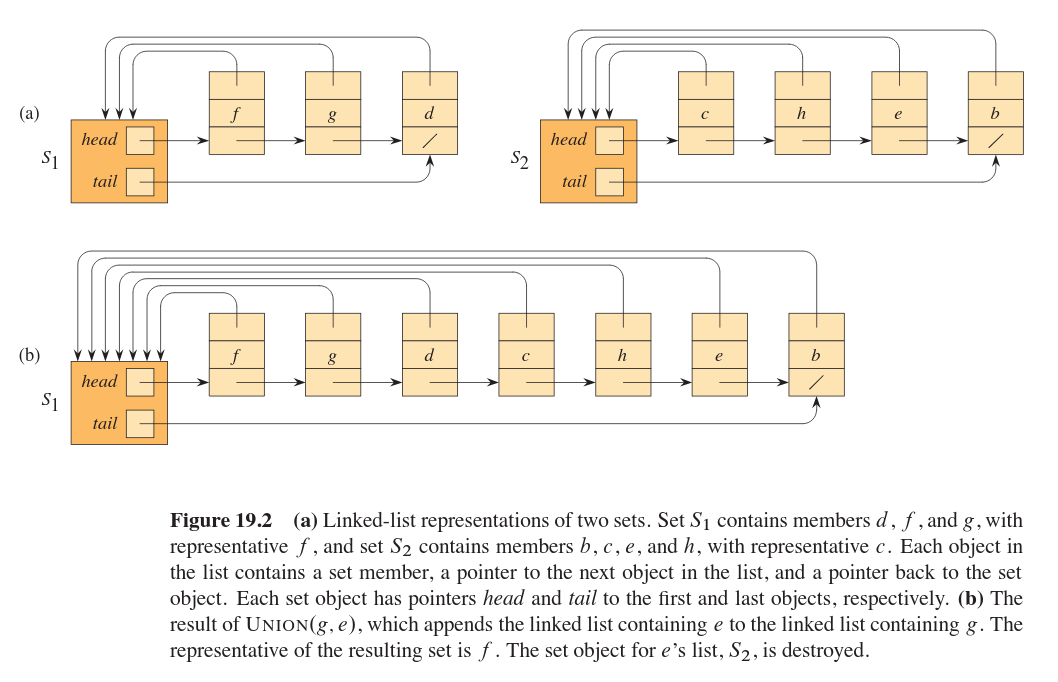
\includegraphics[width=\textwidth]{linked-list.png}
    \end{figure}

    What's the time complexity here for our operations?

    \texttt{MAKE-SET(v)}: $O(1)$, just make a new set with only a single element

    \texttt{FIND-SET(v)}: $O(1)$, just follow the pointer back to the head
    
    \texttt{UNION(u,v)}: $O(n^2)$.

    Union is paying the price for constant-time Find-Set. When two sets are joined, $n$ new pointers must be created that point back to the head. You must do $n$ Make-Set operations, and then a sequence of increasingly long unions that end up summing to $n^2$. This can be amortized away to $n$, but whenever we see an $n^2$ a natural thing to ask is, could this be $n \log n$?

    We can improve on this a little bit by taking the heuristic that we will always add a shorter list to a longer list, but this could still take $\Omega(n)$ time if both sets have the same number of members. 

    Of course we aren't just randomly creating unions; we are creating new sets with Make-Set and then creating unions to existing sets, so in practice we would really like to know what the time complexity is of the Make-Set and Union operations in conjunction with one another. 

    Let's determine an upper bound on the number of times an object's pointer back to its representative is updated. Consider an object $x$. When $x$ is updated, it must have started in the smaller set. The first time $x$ is updated, then, the resulting set must have at least 2 members. Therefore, the next time it is updated, the resulting set must have at least 4 members. Then 8, then 16, and so on.

    For any $k \leq n$, after $x$'s pointer has been updated $\log_2(k)$ times, the resultant set must have at least $k$ members. Since the largest set has at most $n$ members, each object's pointer is updated at most $\log_2(n)$ times over all the Union operations.

    Updating the tails and lengths of lists take linear time, so the total time for Union is $O(n\log n)$. Amortized, we get $\log n$, our favorite runtime.

    \subsection*{Disjoint Set Forests}

    Currently we have a Make-Set operation running in constant time, a Find-Set operation running in constant time, and a Union operation running in $n \log n$ time, leading to an overall runtime of $O(m + n \log n)$. We naturally might want to know if there is a way to improve upon this runtime. 

    The obvious way is to see if we can avoid rearranging all our pointers every time. Whenever a linked list fails us, we tend to turn our attention instead towards trees and see what that can do. 

    \begin{figure}[h]
        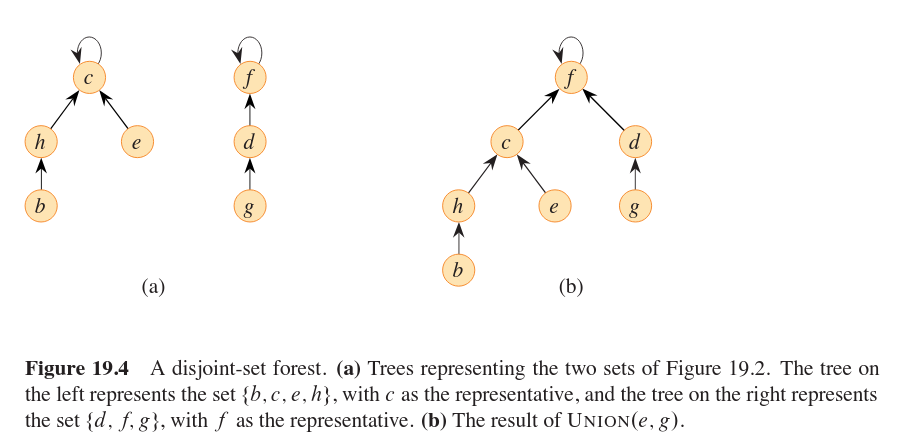
\includegraphics[width=\textwidth]{disjoint-forest.png}
    \end{figure}

    At first glance, this doesn't really improve upon our runtime at all. We've just swapped constant-time union for exponential find! But the power comes in using some heuristics to more intelligently build these trees, and therefore create structures with tighter bounds for search. 

    \subsubsection*{Union by Rank}

    Like before, we join a smaller tree to a larger tree, so that we don't end up with long lists. However, taking the height of a tree is itself an $O(n)$ operation, so we want to avoid having to do that every time. 

    We instead maintain a value \texttt{x.rank} for every node. This rank is an upper bound on the height of $x$. 

    When we start with a single element, x.rank = 0. Find-Set changes nothing; we're just looking at the ranks. 

    For each Union operation, if the roots have unequal ranks, make the root with higher rank the parent of the root with lower rank. If they have equal ranks, choose any one and increment its rank. 

    The reason this is sufficient is because we are never destroying edges, only building them. So we can only go up from 0. And we are always starting with just a single element, so slowly building in this way will work out for us. 

    That's helpful, but it still seems like we're going to have to search every single node to do a Find-Set, which is still $O(n)$. We can improve upon that with something called Path Compression. 

    \subsubsection*{Path Compression}

    Path compression relies on the use of the Find-Set procedure. It is a recursive procedure where we take one pass up a path from the node of interest to find the root. Then, it makes a second pass downward to point each node directly at the root. 

    Why is this a feasible algorithm? Because we are implementing it each time we create a union, we are never going to get an extremely long branching tree. 

    \subsubsection*{Algorithm for Disjoint Set Forest}

    Here is the full pseudocode algorithm for implmentation of a disjoint set forest. Note the operation \texttt{LINK}, which is essentially the union operation on the roots of two elements.

    Note also that $x.p$ is the representative, or root, of the tree that contains $x$.

    \begin{verbatim}
        MAKE-SET(x)
            x.p = x

        UNION(x, y)
            LINK(FIND-SET(x), FIND-SET(y))

        LINK(x, y)
            if x.rank > y.rank              // if the tree with x is larger than that with y
                y.p = x                     // Make x the new root of y
            else x.p = y                    // otherwise make y the new root of x
                if x.rank == y.rank         // and if the ranks are equal, increment y's rank
                    y.rank = y.rank + 1

        
        FIND-SET(x)
            if x != x.p                     // are we at the root? if not,
                x.p = FIND-SET(x.p)           // the root becomes the parent of x
            return x.p                      // then return the root
    \end{verbatim}


    \subsection*{Analysis of Runtime}

    This is all well and good, but how much does this actually help us?

    The union by rank gives a runtime of $O(m \log n)$ for $m$ operations; while we won't show it here, this should sound intuitively true based on the fact that it certainly can't be any \textit{worse} than the linear approach.

    The path compression by itself for a sequence of $n$ Make-Set operations and $k$ find-set operations gives a worst-case runtime of $\Theta(n + k(1 + \log_{2+f/n}n))$. 

    The combination of the two gives a runtime of $O(m\alpha(n))$, where $\alpha(n)$ is a very slow-growing function. In practical terms, $\alpha(n) \leq 4$, but in the theoretical case it could be larger. Therefore we can't say the runtime is technically linear in $m$, but for practical purposes, it basically is. 

    The proof of this entire runtime is about 8 pages long in your book, so we aren't going to do it in class. But for a very, very quick explanation of what makes $\alpha(n)$ so slow-growing, it has to do with how many layers out from the root you would need to go in order to have a really bad path compression step (a lot). 

\end{document}